\section{ROS}

In this section, the current structure of the separate components will be explained.
Not all of how ROS works is understood by this group, since it was not built from the ground up by the 2019 Q1\&Q2 group, but an attempt has been made to document it nonetheless.

\begin{figure}[H]
\centering
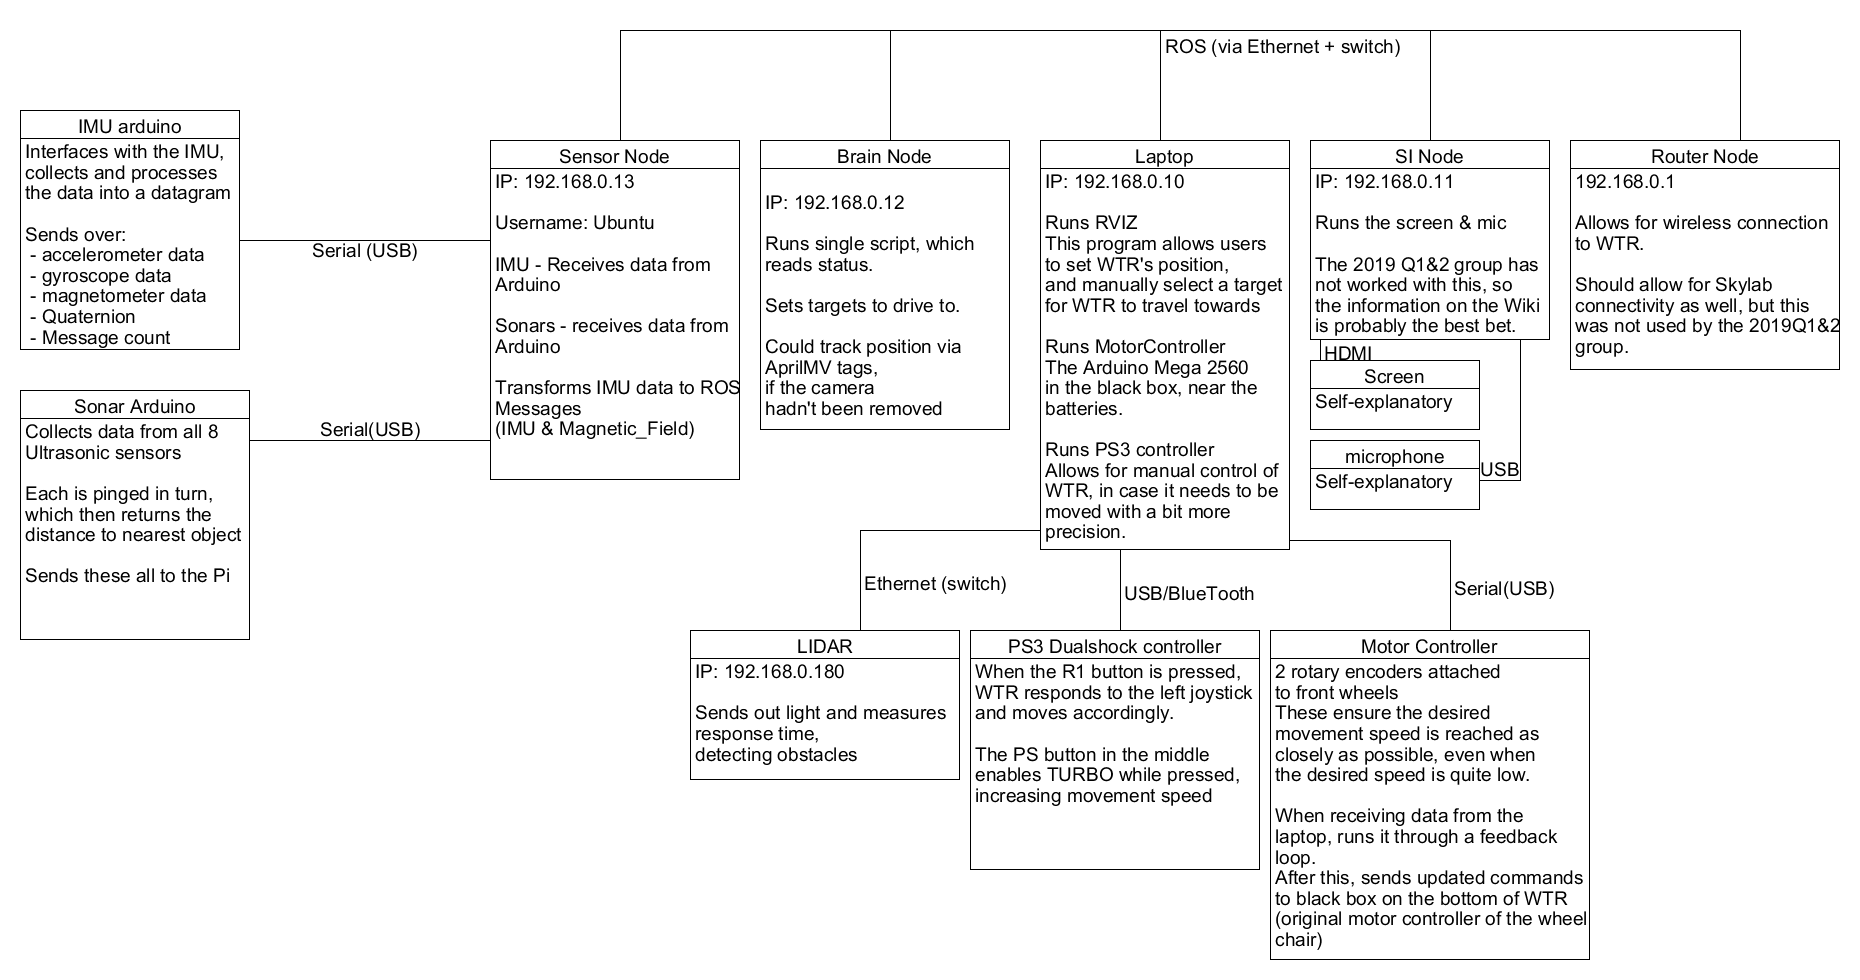
\includegraphics[width=15cm]{ROSoverview.png}
\caption{An overview of every programmable/relevant component}
\label{fig::ROSover}
\end{figure}

In figure \ref{fig::ROSover}, each block represents a device or component used.
Since the group did not work on the social interaction (SI node), Skylab (used with the Router node/Brain node), the documentation on those will be less than optimal.
Each line represents the method through which the devices communicate, such as Serial communication over a USB connection.

Inside the nodes are brief explanations of what each device or component does.
More detailed explanations of functionality worked on can be found in their specific sections.
\newpage